\section{Energy Class Reference}
\label{classEnergy}\index{Energy@{Energy}}
{\tt \#include $<$energy.h$>$}

Collaboration diagram for Energy:\begin{figure}[H]
\begin{center}
\leavevmode
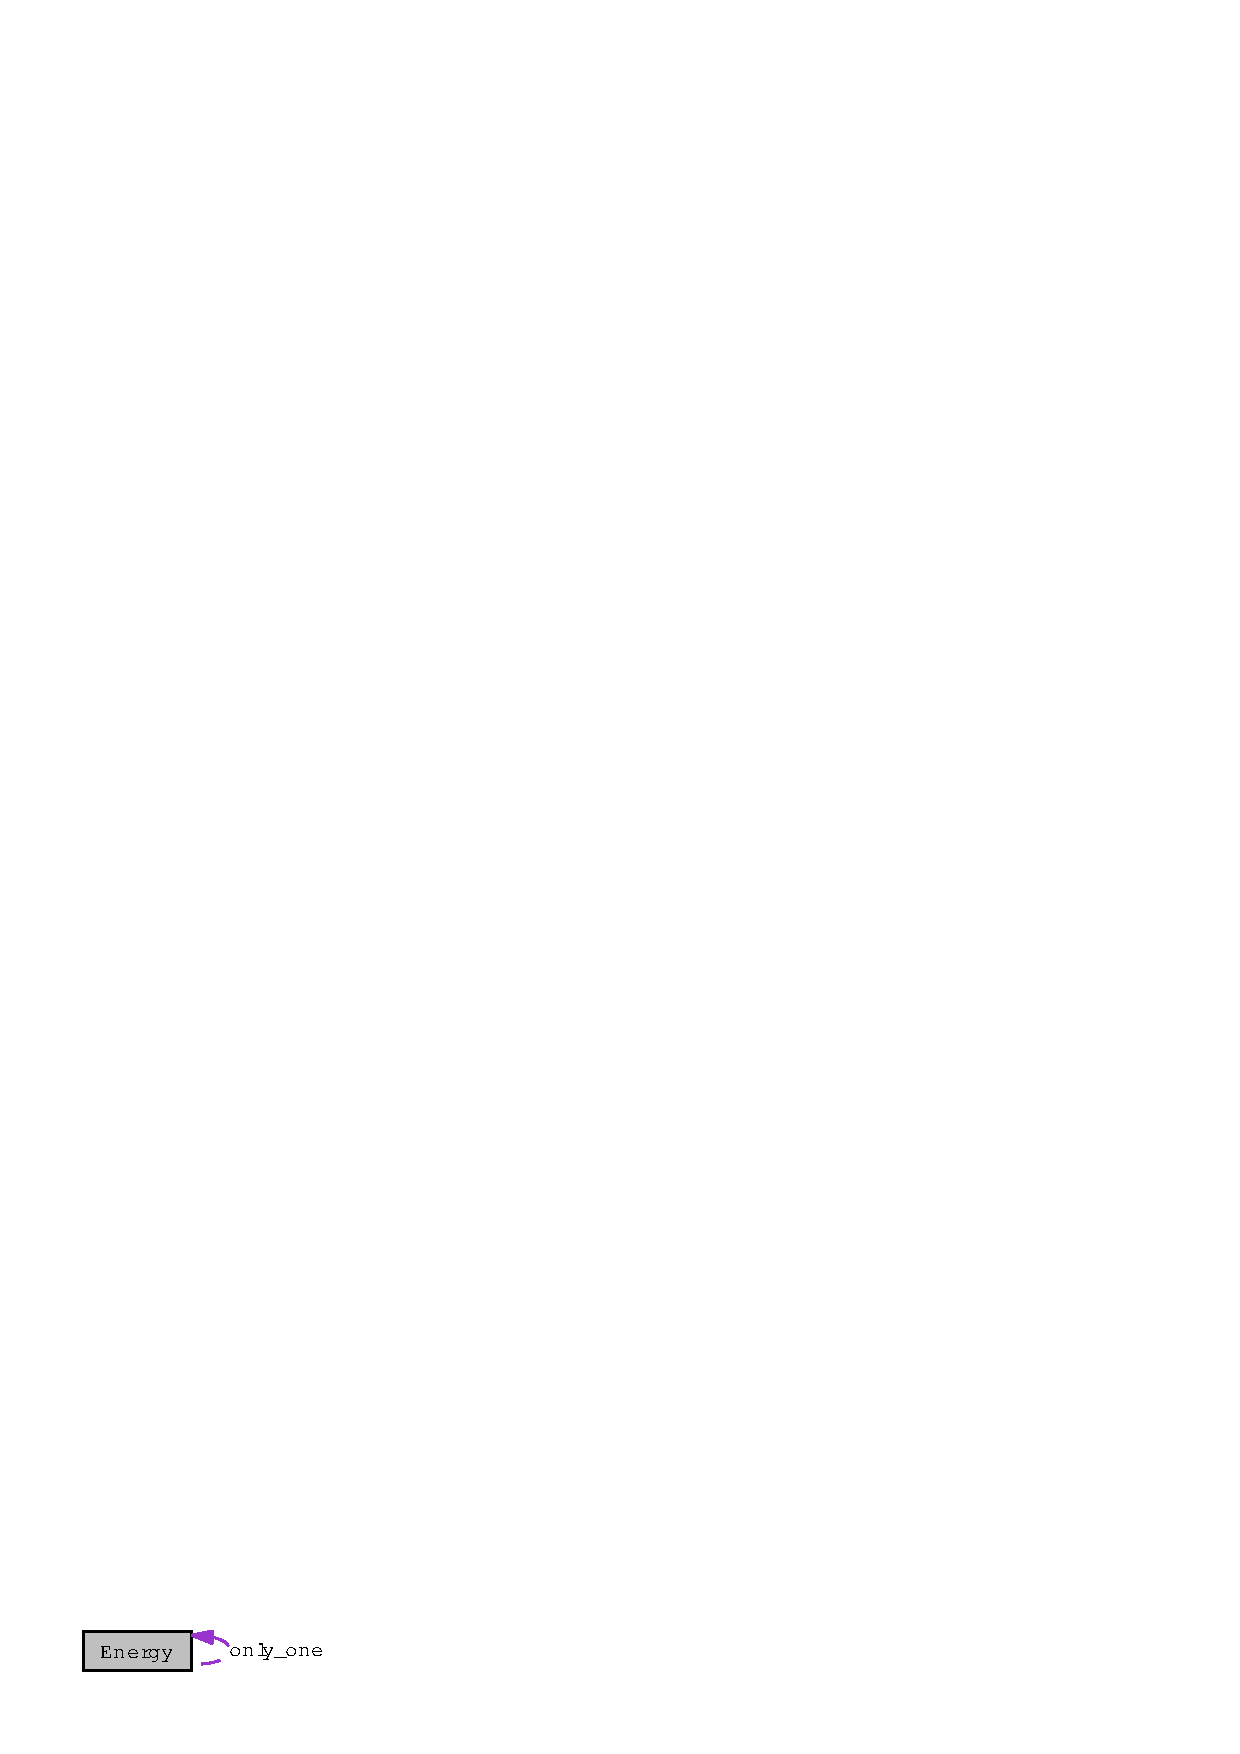
\includegraphics[width=80pt]{classEnergy__coll__graph}
\end{center}
\end{figure}
\subsection*{Public Member Functions}
\begin{CompactItemize}
\item 
void {\bf compute\-Global\-Energy} (void)
\item 
void {\bf write\-Stats} (std::ostream \&)
\end{CompactItemize}
\subsection*{Static Public Member Functions}
\begin{CompactItemize}
\item 
static {\bf Energy} \& {\bf instance} (void)
\end{CompactItemize}


\subsection{Member Function Documentation}
\index{Energy@{Energy}!instance@{instance}}
\index{instance@{instance}!Energy@{Energy}}
\subsubsection{\setlength{\rightskip}{0pt plus 5cm}{\bf Energy} \& Energy::instance (void)\hspace{0.3cm}{\tt  [static]}}\label{classEnergy_0507547be610702ae317b136fd05c31d}


\index{Energy@{Energy}!computeGlobalEnergy@{computeGlobalEnergy}}
\index{computeGlobalEnergy@{computeGlobalEnergy}!Energy@{Energy}}
\subsubsection{\setlength{\rightskip}{0pt plus 5cm}void Energy::compute\-Global\-Energy (void)}\label{classEnergy_fe2e06beeb8f6cadb07bfbd2f8a1d96e}


\index{Energy@{Energy}!writeStats@{writeStats}}
\index{writeStats@{writeStats}!Energy@{Energy}}
\subsubsection{\setlength{\rightskip}{0pt plus 5cm}void Energy::write\-Stats (std::ostream \& {\em target})}\label{classEnergy_818c911e57dd9c7d7be0c8b22f2f1957}


Print total model energy statistics.

\begin{Desc}
\item[Parameters:]
\begin{description}
\item[\mbox{$\leftarrow$} {\em target}]Pre-initialized output stream. \end{description}
\end{Desc}


The documentation for this class was generated from the following files:\begin{CompactItemize}
\item 
{\bf energy.h}\item 
{\bf energy.cc}\end{CompactItemize}
